\chapter{Experiment and Result}
\label{c:Experiment-and-Result}




\if 0
\bibliography{thesis}
\graphicspath{{./figsrc/}}
\fi

\section{DEMO}
We have briefly shown user flow of all user cases in previous chapter. In this section, we will show what it looks like in Front-end(web page) perspective in every steps of sequence diagram we mentioned in Chapter 3.

% 4 個 Case 展示
\subsection{Manual record}
Video DEMO: https://www.youtube.com/watch?v=HOrxz-9iKsw
 
In manual case, we will show the situation in Front-end happend in Fig.~\ref{fig:manual-sequece-diagram}. First, we click recording button at the streaming web page as shown in Fig.~\ref{fig:demo-manual-1}. Fig.~\ref{fig:demo-manual-2} will start to ask PI for permission. If we get permission, it will start building WebSocket connection and Recording server will start connecting to Video streaming server as shown in Fig.~\ref{fig:demo-manual-3}. When Recording server finishes connecting to Video streaming server, web-page will get informed that the recording process has begun as shown in Fig.~\ref{fig:demo-manual-4}. User clicks stop button in Fig.~\ref{fig:demo-manual-5} to terminate recording process. We can find file in AWS S3 as shown in youtube DEMO.

\begin{figure}[H]
    \ContinuedFloat
    \centering
    \begin{subfigure}{\textwidth}
        \includegraphics[width=\textwidth]{figsrc/demo-manual-1.png}
        \subcaption{Click start button}
        \label{fig:demo-manual-1}
    \end{subfigure}
\end{figure}

\begin{figure}[H]
    \ContinuedFloat
    \centering
    \begin{subfigure}{\textwidth}
        \includegraphics[width=\textwidth]{figsrc/demo-manual-2.png}
        \subcaption{Wait for permission}
        \label{fig:demo-manual-2}
    \end{subfigure}
\end{figure}

\begin{figure}[H]
    \ContinuedFloat
    \centering
    \begin{subfigure}{\textwidth}
        \includegraphics[width=\textwidth]{figsrc/demo-manual-3.png}
        \subcaption{Wait for connection}
        \label{fig:demo-manual-3}
    \end{subfigure}
\end{figure}

\begin{figure}[H]
    \ContinuedFloat
    \centering
    \begin{subfigure}{\textwidth}
        \includegraphics[width=\textwidth]{figsrc/demo-manual-4.png}
        \subcaption{Start recording}
        \label{fig:demo-manual-4}
    \end{subfigure}
\end{figure}


\begin{figure}[H]
    \ContinuedFloat
    \centering
    \begin{subfigure}{\textwidth}
        \includegraphics[width=\textwidth]{figsrc/demo-manual-5.png}
        \subcaption{Stop recording}
        \label{fig:demo-manual-5}
    \end{subfigure}

    \caption{DEMO of manual case}
    \label{fig:demo-manual}
\end{figure}

% time triggered(event trigger那邊平台還沒做好)
\subsection{Triggered based record}
Video DEMO: https://www.youtube.com/watch?v=yN4NbbG5he4

We will show the situation of sequence diagram of Fig.~\ref{fig:time-sequence-diagram} that happened in Front-end. We first set, duration, angle and the timing to record at 1:39PM, one minute later in Fig.~\ref{fig:demo-time-1}. At this moment, Scheduling server will recieve new setting that waits to execute. When time's up, scheduling server will reuqest PI to record. PI turns the camera from Fig.~\ref{fig:demo-time-2} to Fig.~\ref{fig:demo-time-3} at video timestamp 1:00\~1:05 then orders recording server to start the process.

\begin{figure}[H]
    \centering
    \begin{subfigure}{\textwidth}
        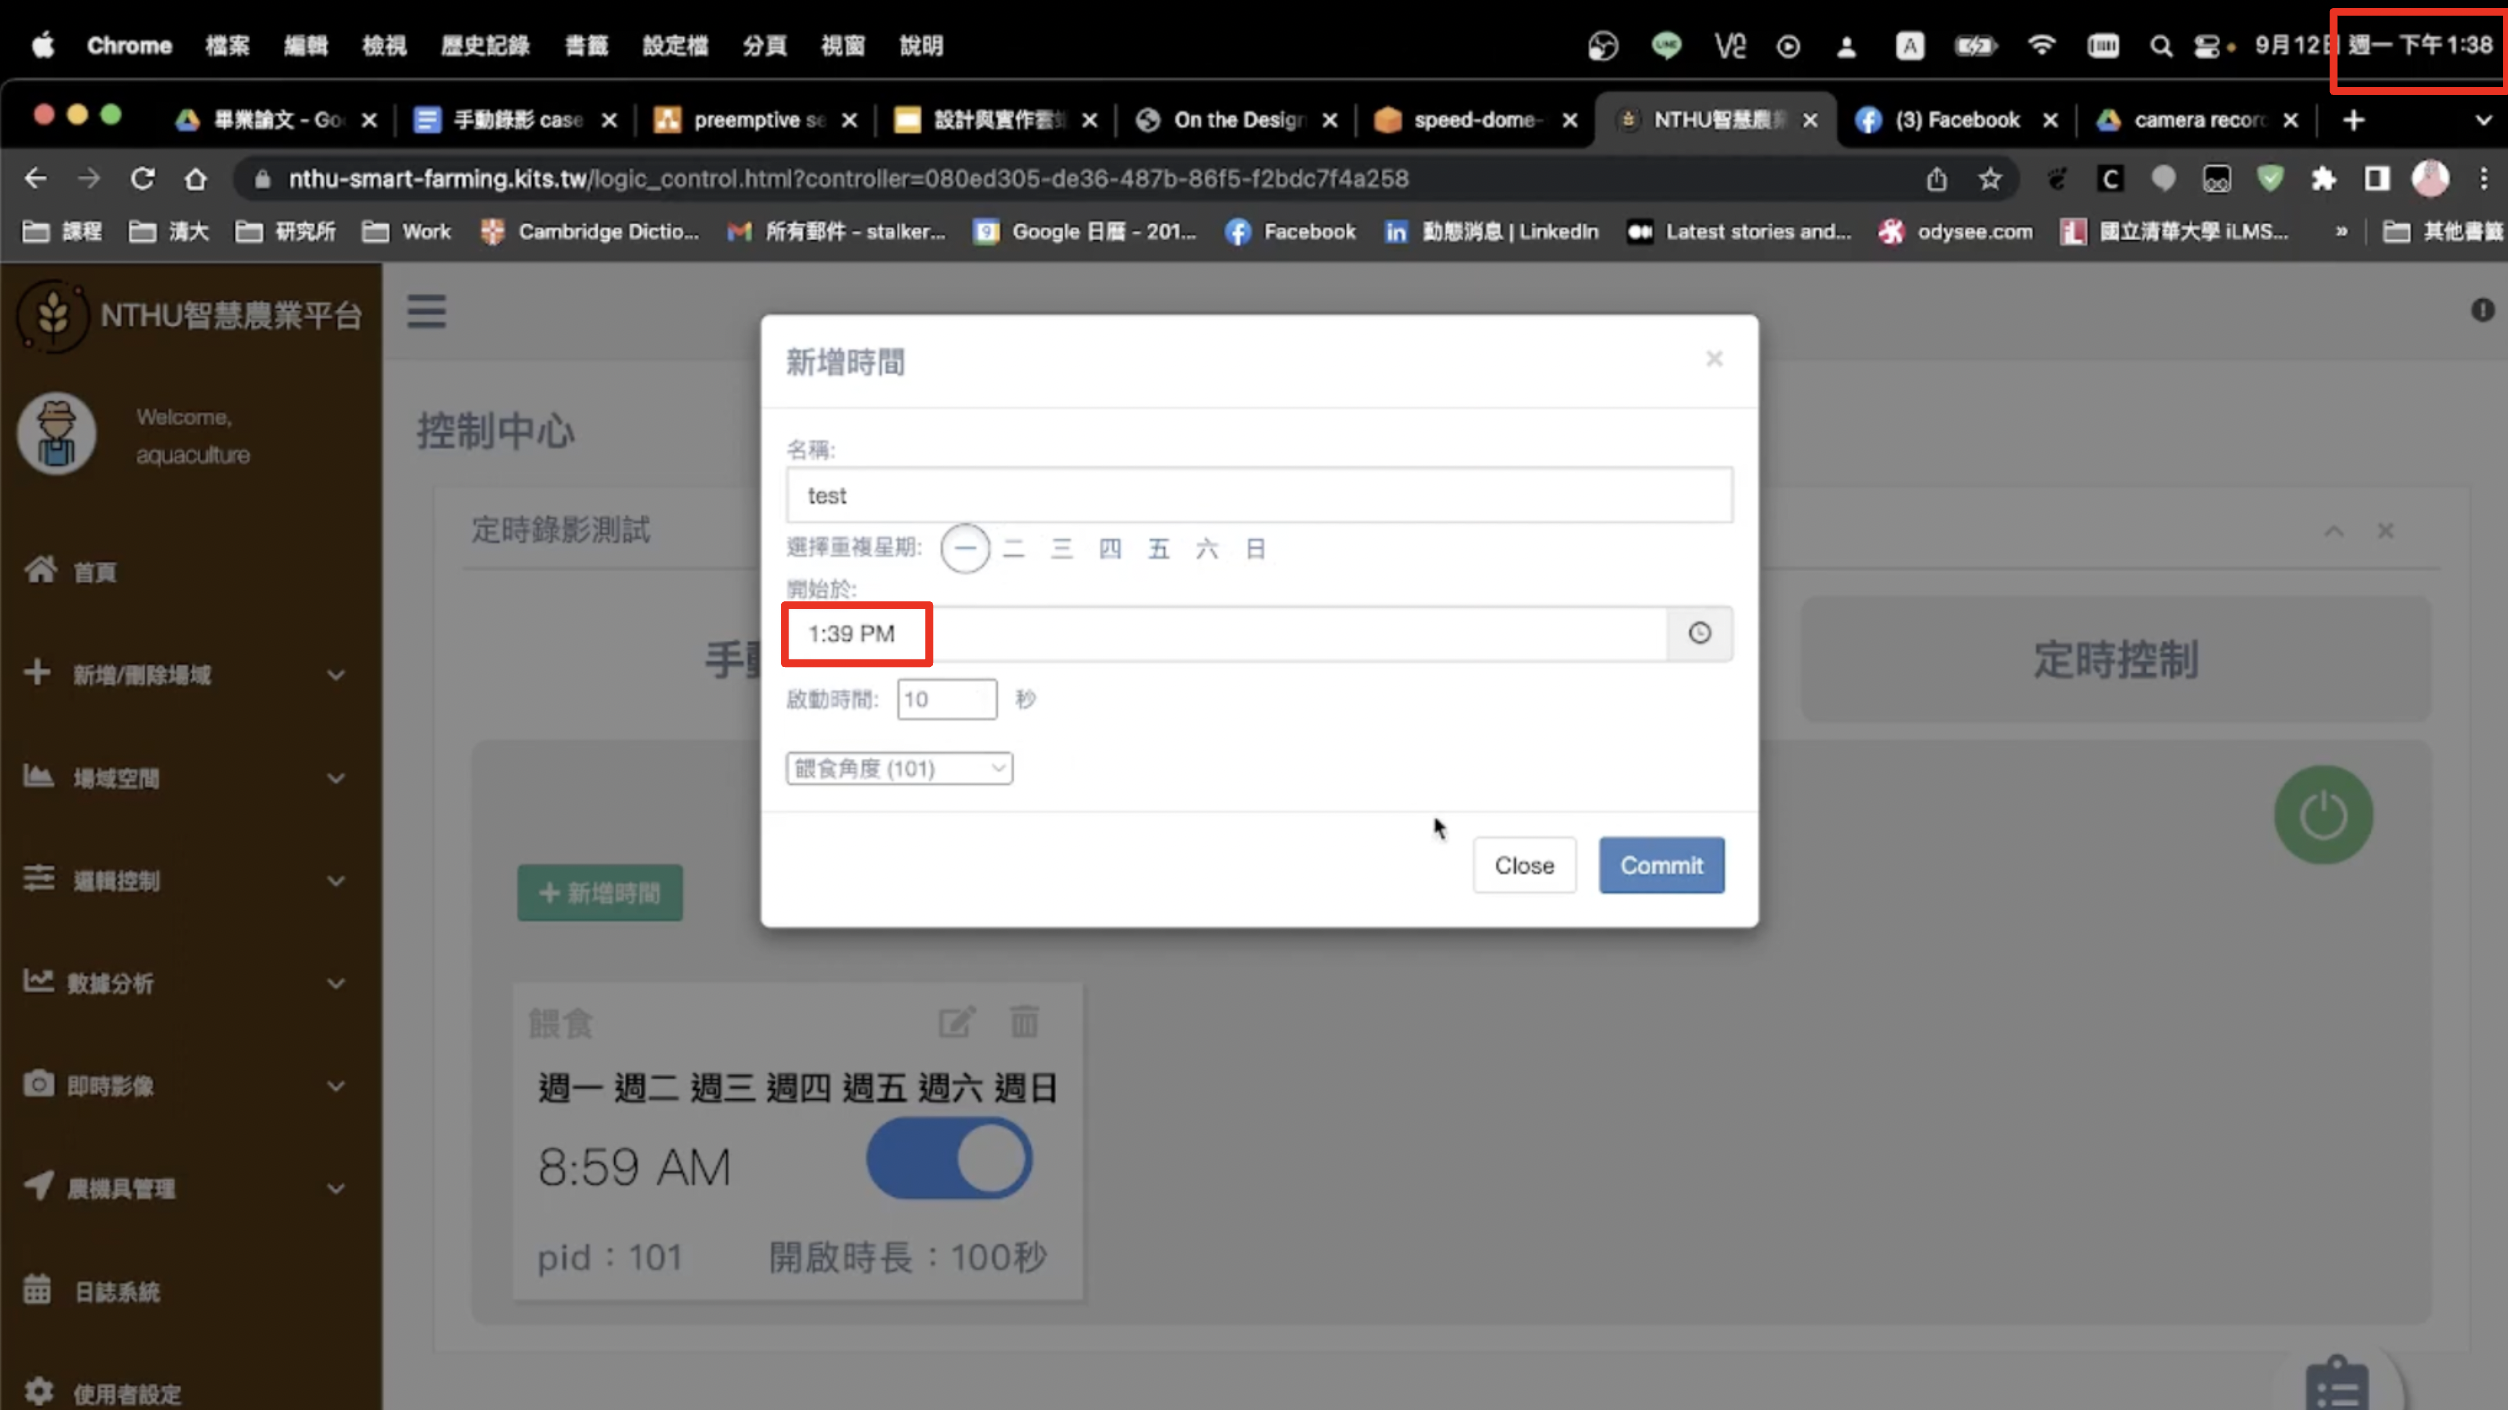
\includegraphics[width=\textwidth]{figsrc/demo-time-1.png}
        \subcaption{Set time schedule}
        \label{fig:demo-time-1}
    \end{subfigure}
\end{figure}


\begin{figure}[H]
    \ContinuedFloat
    \centering
    \begin{subfigure}{\textwidth}
        \includegraphics[width=\textwidth]{figsrc/demo-time-2.png}
        \subcaption{Angle before recording}
        \label{fig:demo-time-2}
    \end{subfigure}
\end{figure}

\begin{figure}[H]
    \ContinuedFloat
    \centering
    \begin{subfigure}{\textwidth}
        \includegraphics[width=\textwidth]{figsrc/demo-time-3.png}
        \subcaption{Angle after recording}
        \label{fig:demo-time-3}
    \end{subfigure}

    \caption{DEMO of triggered case}
    \label{fig:demo-time}
\end{figure}

% higher preemptive
\subsection{Higher preemptive case}
Video DEMO: https://www.youtube.com/watch?v=\_GLhjjII8Pg

We will show how higher priority task preempt lower priority one in Front-end side. As shown in Fig~\ref{fig:demo-higher-1}, we first set a request that will occur one minute later, then we start manual record in Fig.~\ref{fig:demo-higher-2}. In Fig.~\ref{fig:demo-higher-3}, When time request triggers, we can see in web page that it will stop the recording preocess and send alert to user. At the same time, recording server will upload user's video file to AWS S3 then start new recording task. The preemptive data flow can be saw in Chapter 3 Fig.\ref{fig:preemptive-B-higher}.


\begin{figure}[H]
    \centering
    \begin{subfigure}{\textwidth}
        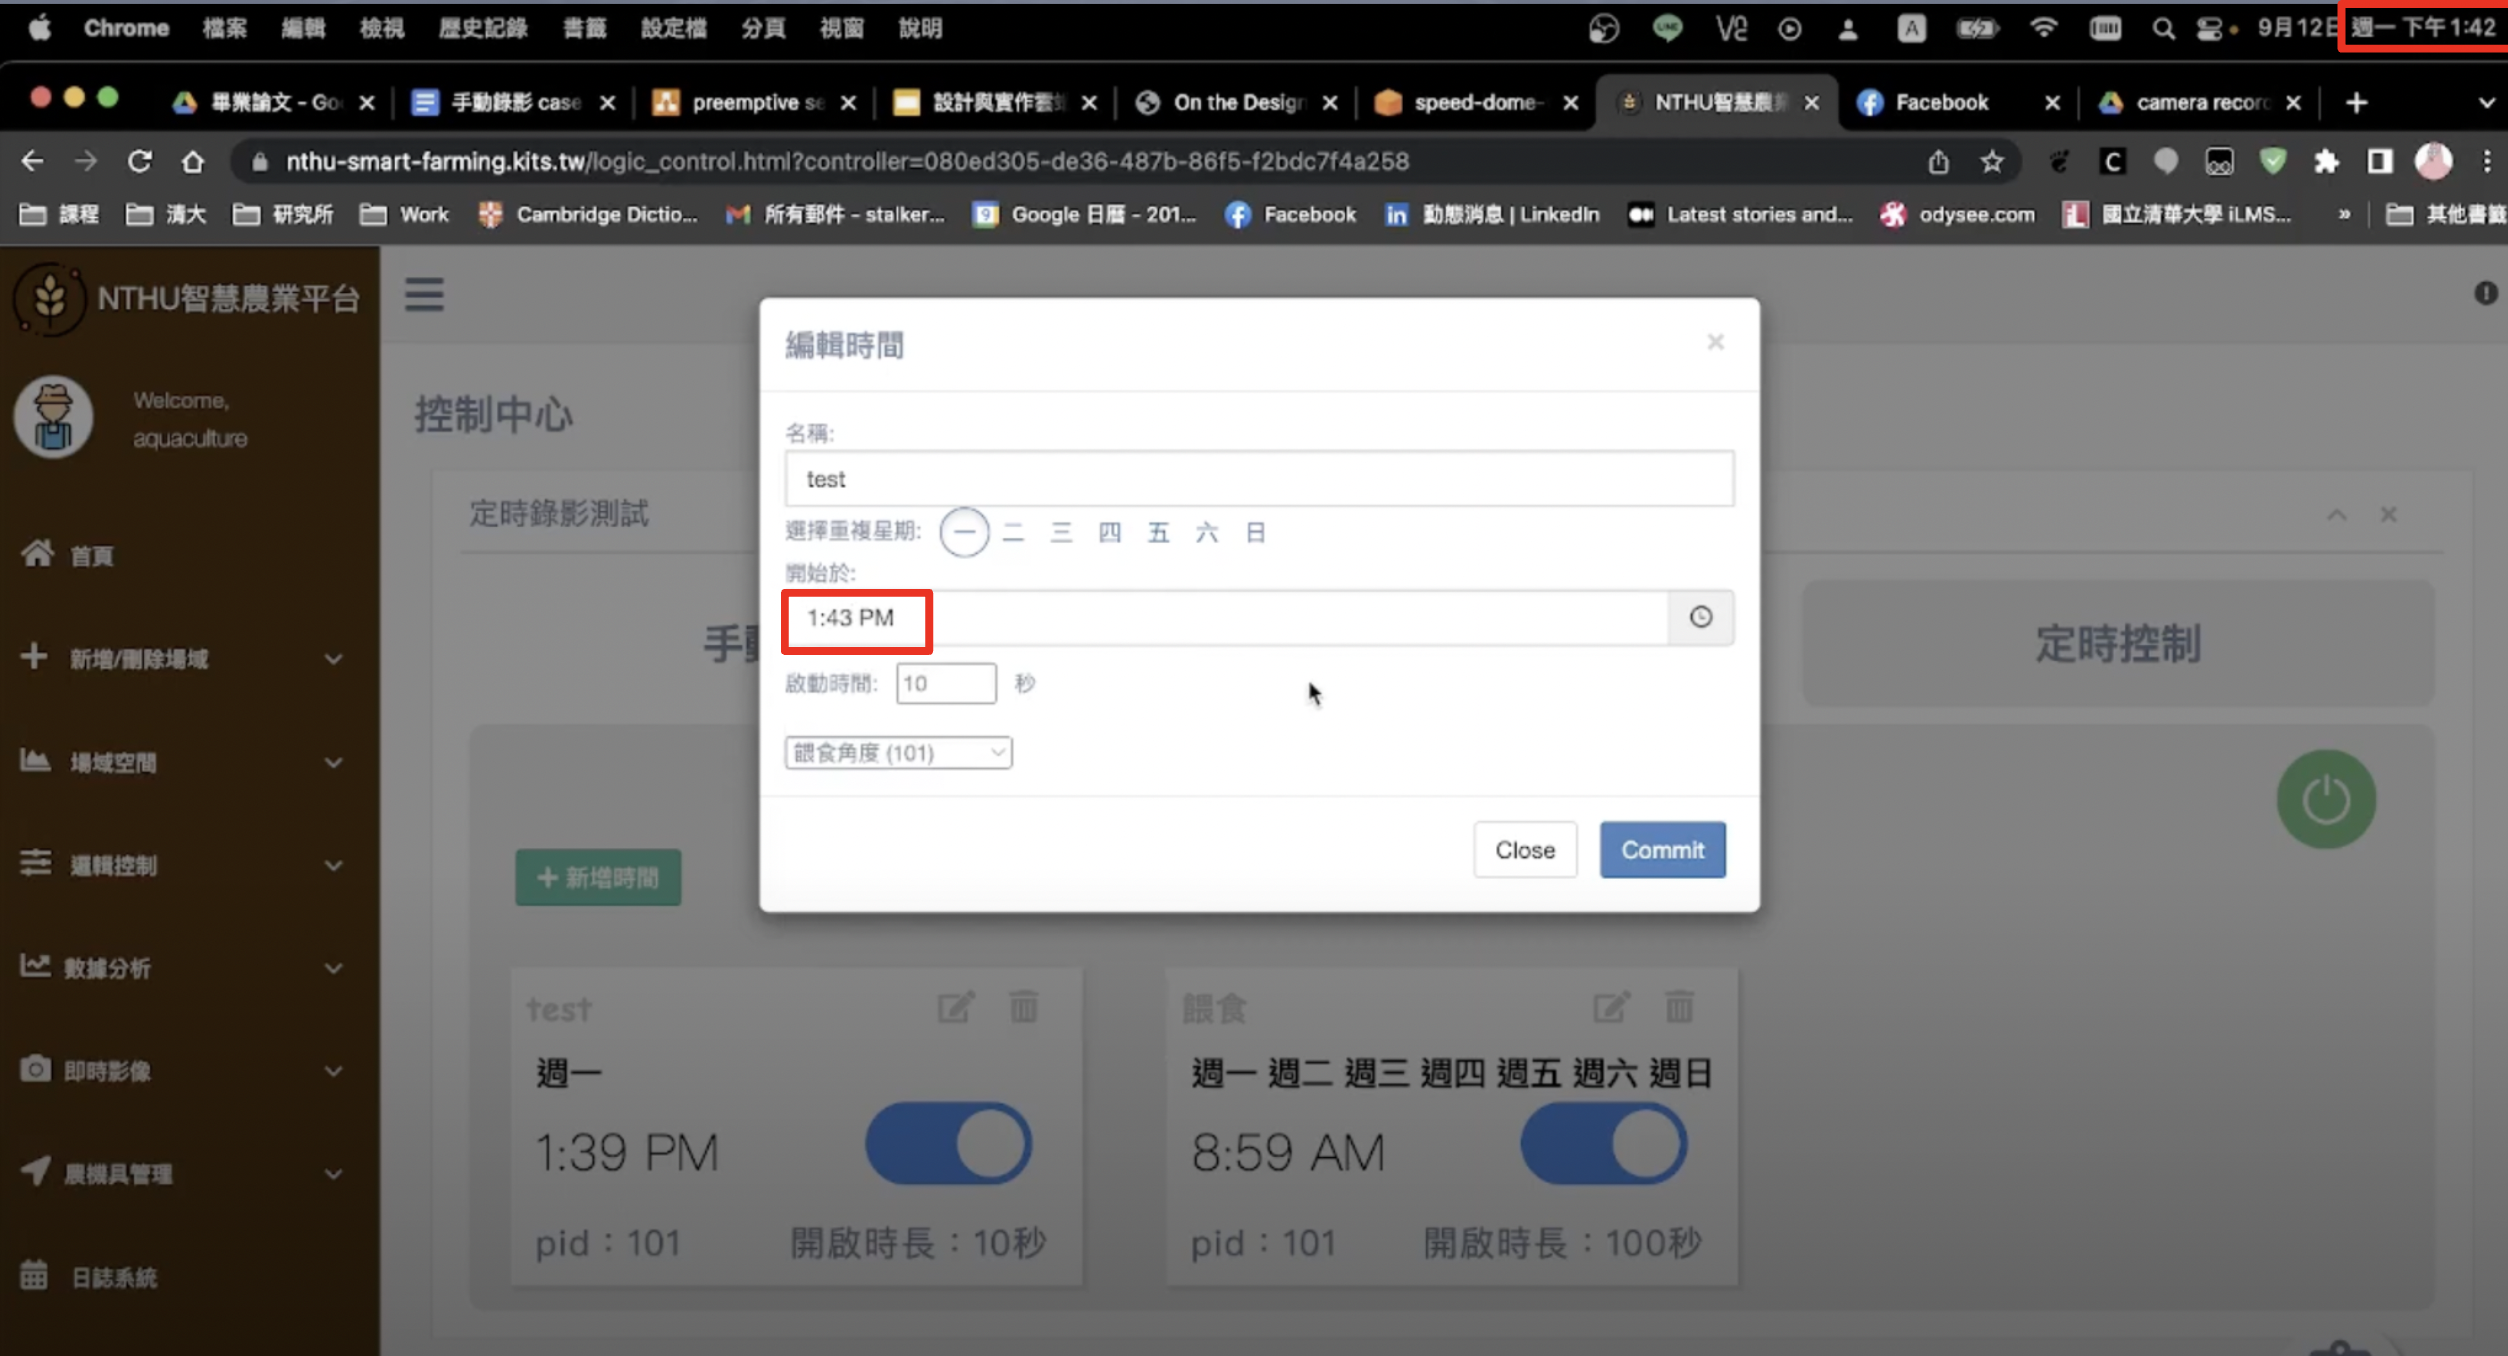
\includegraphics[width=\textwidth]{figsrc/demo-higher-1.png}
        \subcaption{Set time schedule}
        \label{fig:demo-higher-1}
    \end{subfigure}
\end{figure}

\begin{figure}[H]
    \ContinuedFloat
    \centering
    \begin{subfigure}{\textwidth}
        \includegraphics[width=\textwidth]{figsrc/demo-higher-2.png}
        \subcaption{Start manual record}
        \label{fig:demo-higher-2}
    \end{subfigure}
\end{figure}

\begin{figure}[H]
    \ContinuedFloat
    \centering
    \begin{subfigure}{\textwidth}
        \includegraphics[width=\textwidth]{figsrc/demo-higher-3.png}
        \subcaption{New task preempt old task}
        \label{fig:demo-higher-3}
    \end{subfigure}

    \caption{DEMO of higher preemptive case}
    \label{fig:demo-higher}
\end{figure}

\subsection{Lower preemptive case}
Video DEMO: https://www.youtube.com/watch?v=1SY6WzD8WKA

We will show how higher priority task preempt lower priority one in Front-end perspective. In Fig.~\ref{fig:demo-lower-1}, we use two web page to simulate two manual recording request. Leftside of the web page will execute with higher priority by pressing forcing executing button at left down corner. In Fig.~\ref{fig:demo-lower-2}, right side user gets rejection when left side user is occupying the resource since its priority is lower than left side user.

\begin{figure}[H]
    \centering
    \begin{subfigure}{\textwidth}
        \includegraphics[width=\textwidth]{figsrc/demo-lower-1.png}
        \subcaption{Start with higher priority record at left side web page}
        \label{fig:demo-lower-1}
    \end{subfigure}
\end{figure}

\begin{figure}[H]
    \ContinuedFloat
    \centering
    \begin{subfigure}{\textwidth}
        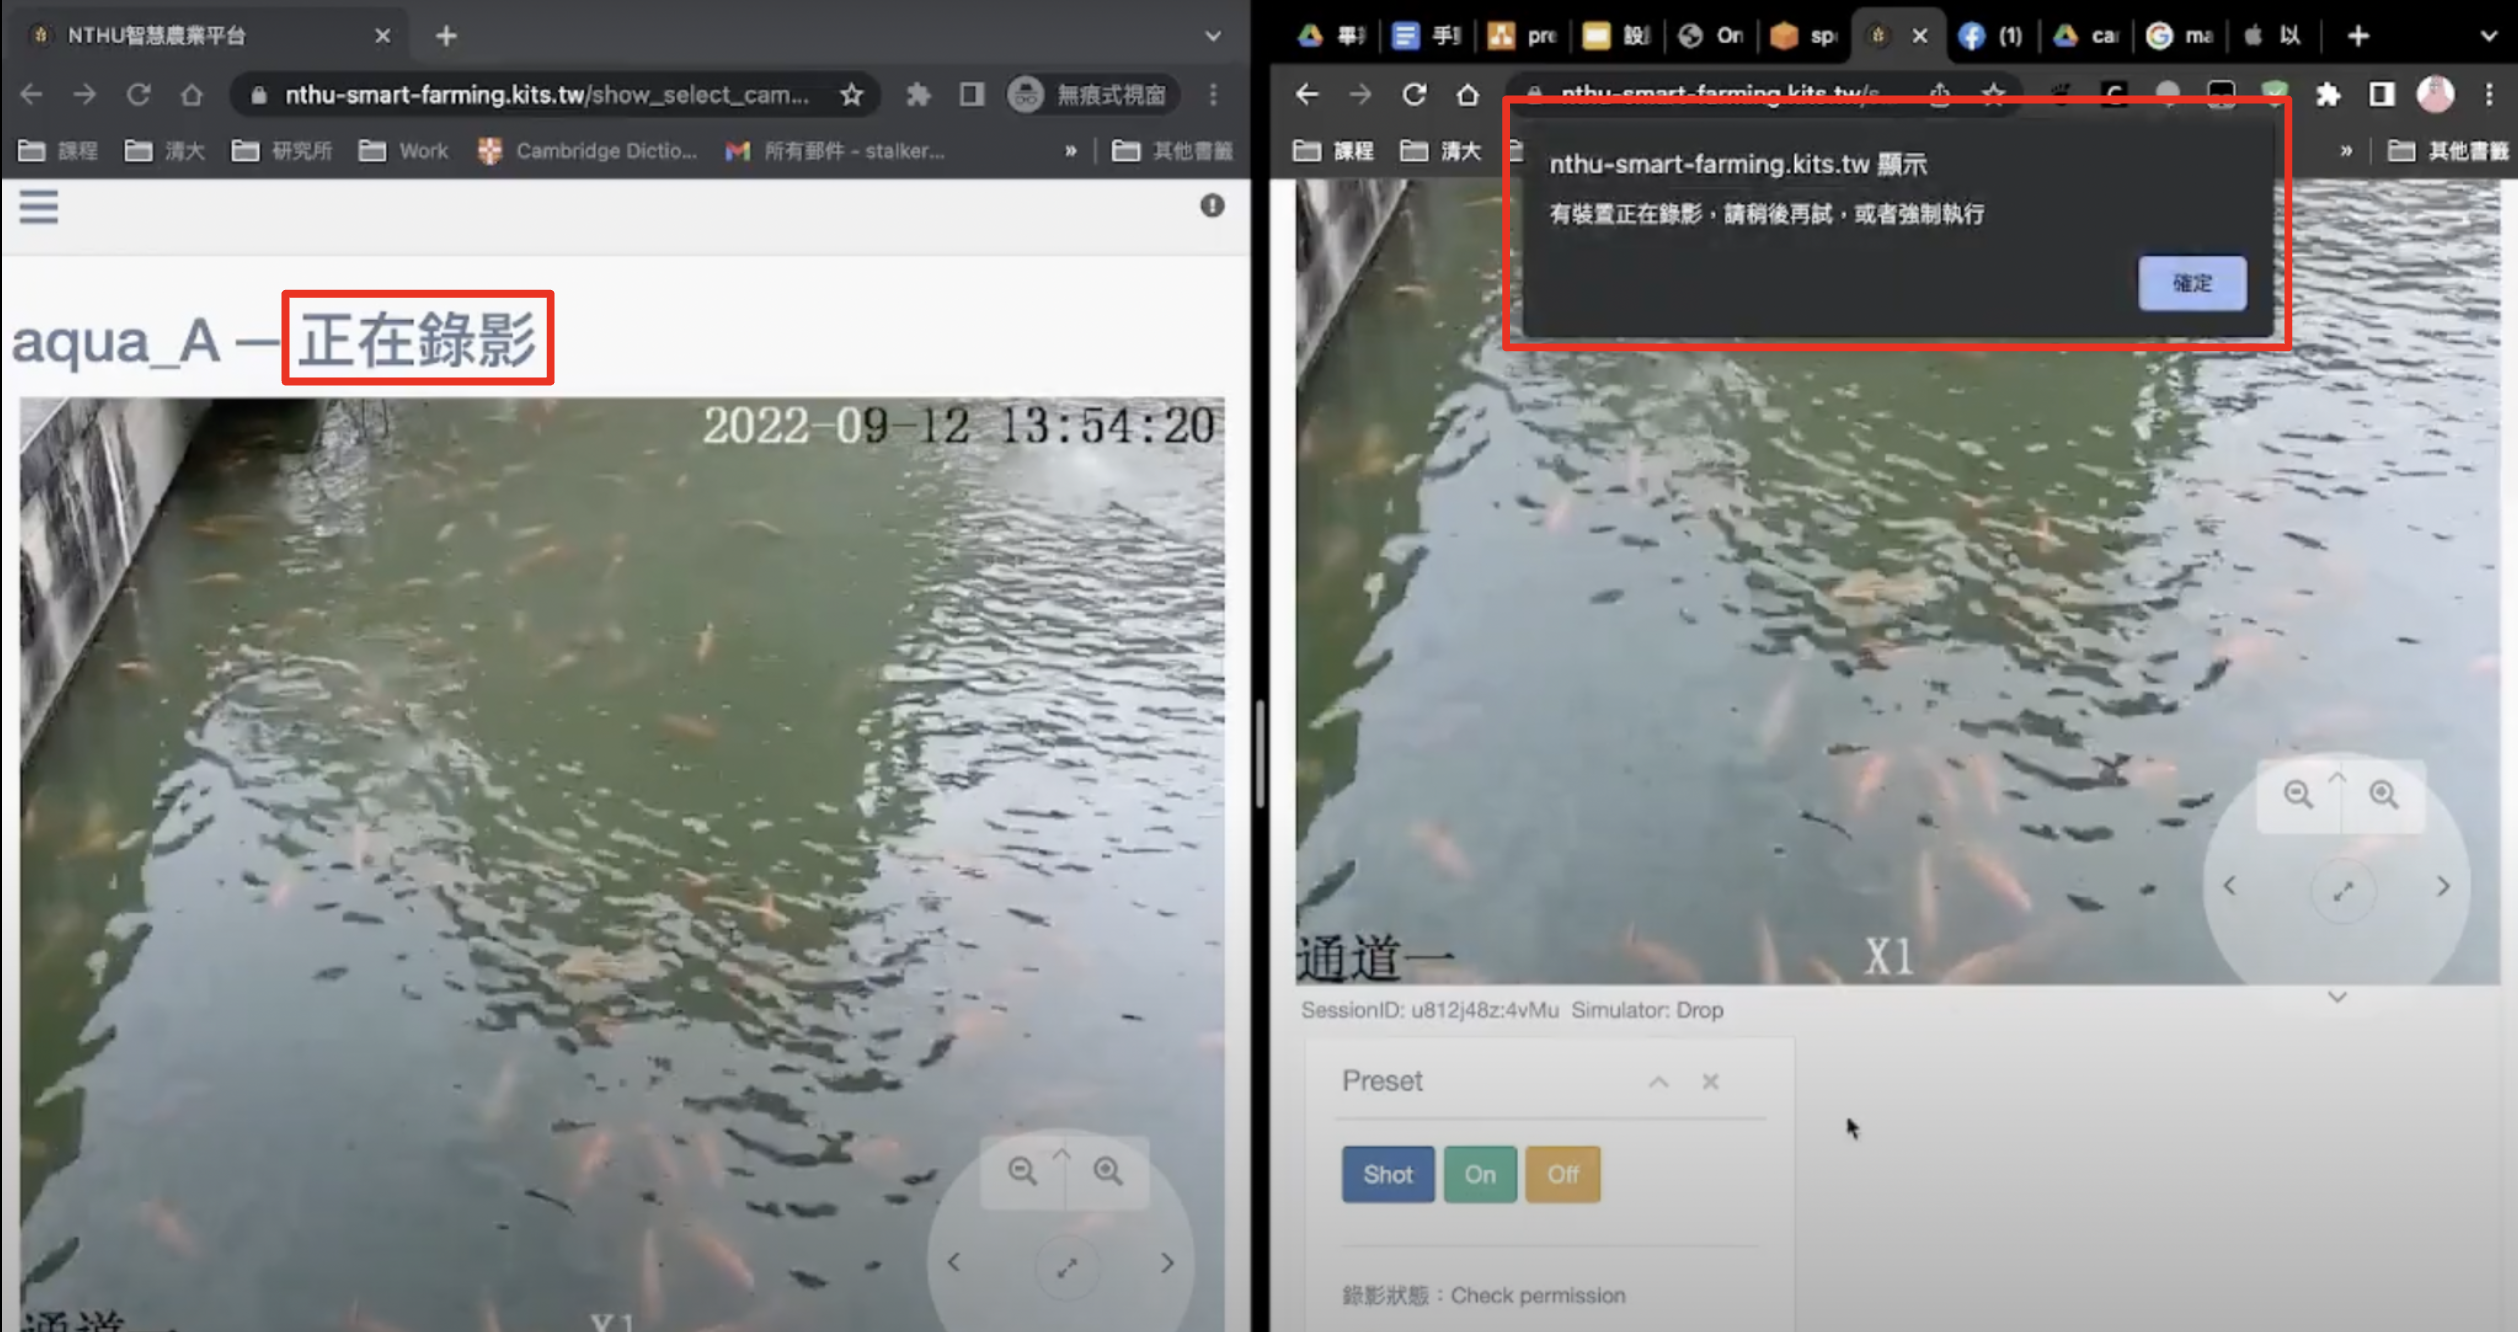
\includegraphics[width=\textwidth]{figsrc/demo-lower-2.png}
        \subcaption{Right side user gets rejection while left side is recording}
        \label{fig:demo-lower-2}
    \end{subfigure}

    \caption{DEMO of lower rejection case}
    \label{fig:demo-lower}
\end{figure}

% 希望之後有像下面影片這樣的應用
% 單一工作效能分析 4階段
\section{Experiment Results}
Here we will measure our system performance. We divide the whole recording process into 4 phases, including permission request, build connection, recording and uploading as shown in Fig.~\ref{fig:result-4phases}. If we don't count preemptive case, we have three major use cases, manual, time period and event trigger. We use manual case to analyze the performance of the system. Because other two cases only have 3 phases, build connection, recording and uploading. They don't have permission request phase.

\begin{figure}[H]
    \centering
    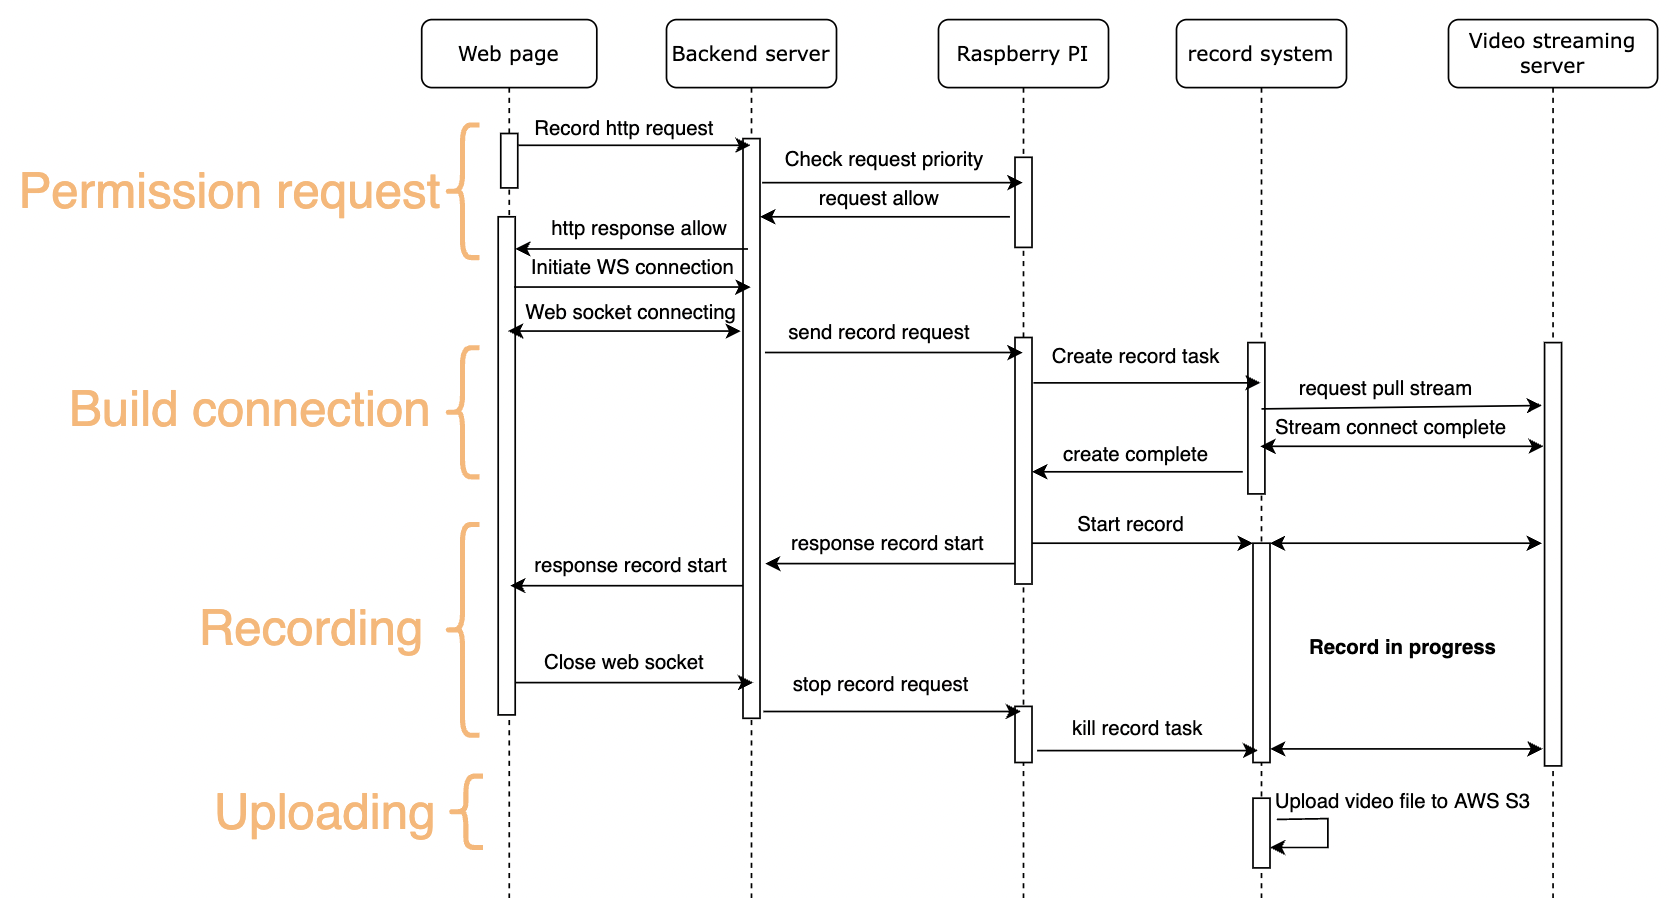
\includegraphics[width=\textwidth]{figsrc/result-4phases.png}
    \caption{4 phases in manual cases\label{fig:result-4phases}}
\end{figure}

% pre
\subsection{Phase 1: Permission request}
In Permission request phase, PI will check whether the user have permission or not. We will measure the time elapsed from http request to http response. We send http request 500 times then get the latency chart below in Fig.~\ref{fig:result-p1}. We can see that the average time elapsed for requesting permission is 902.856ms and STD is 308.034.

\begin{figure}[H]
    \centering
    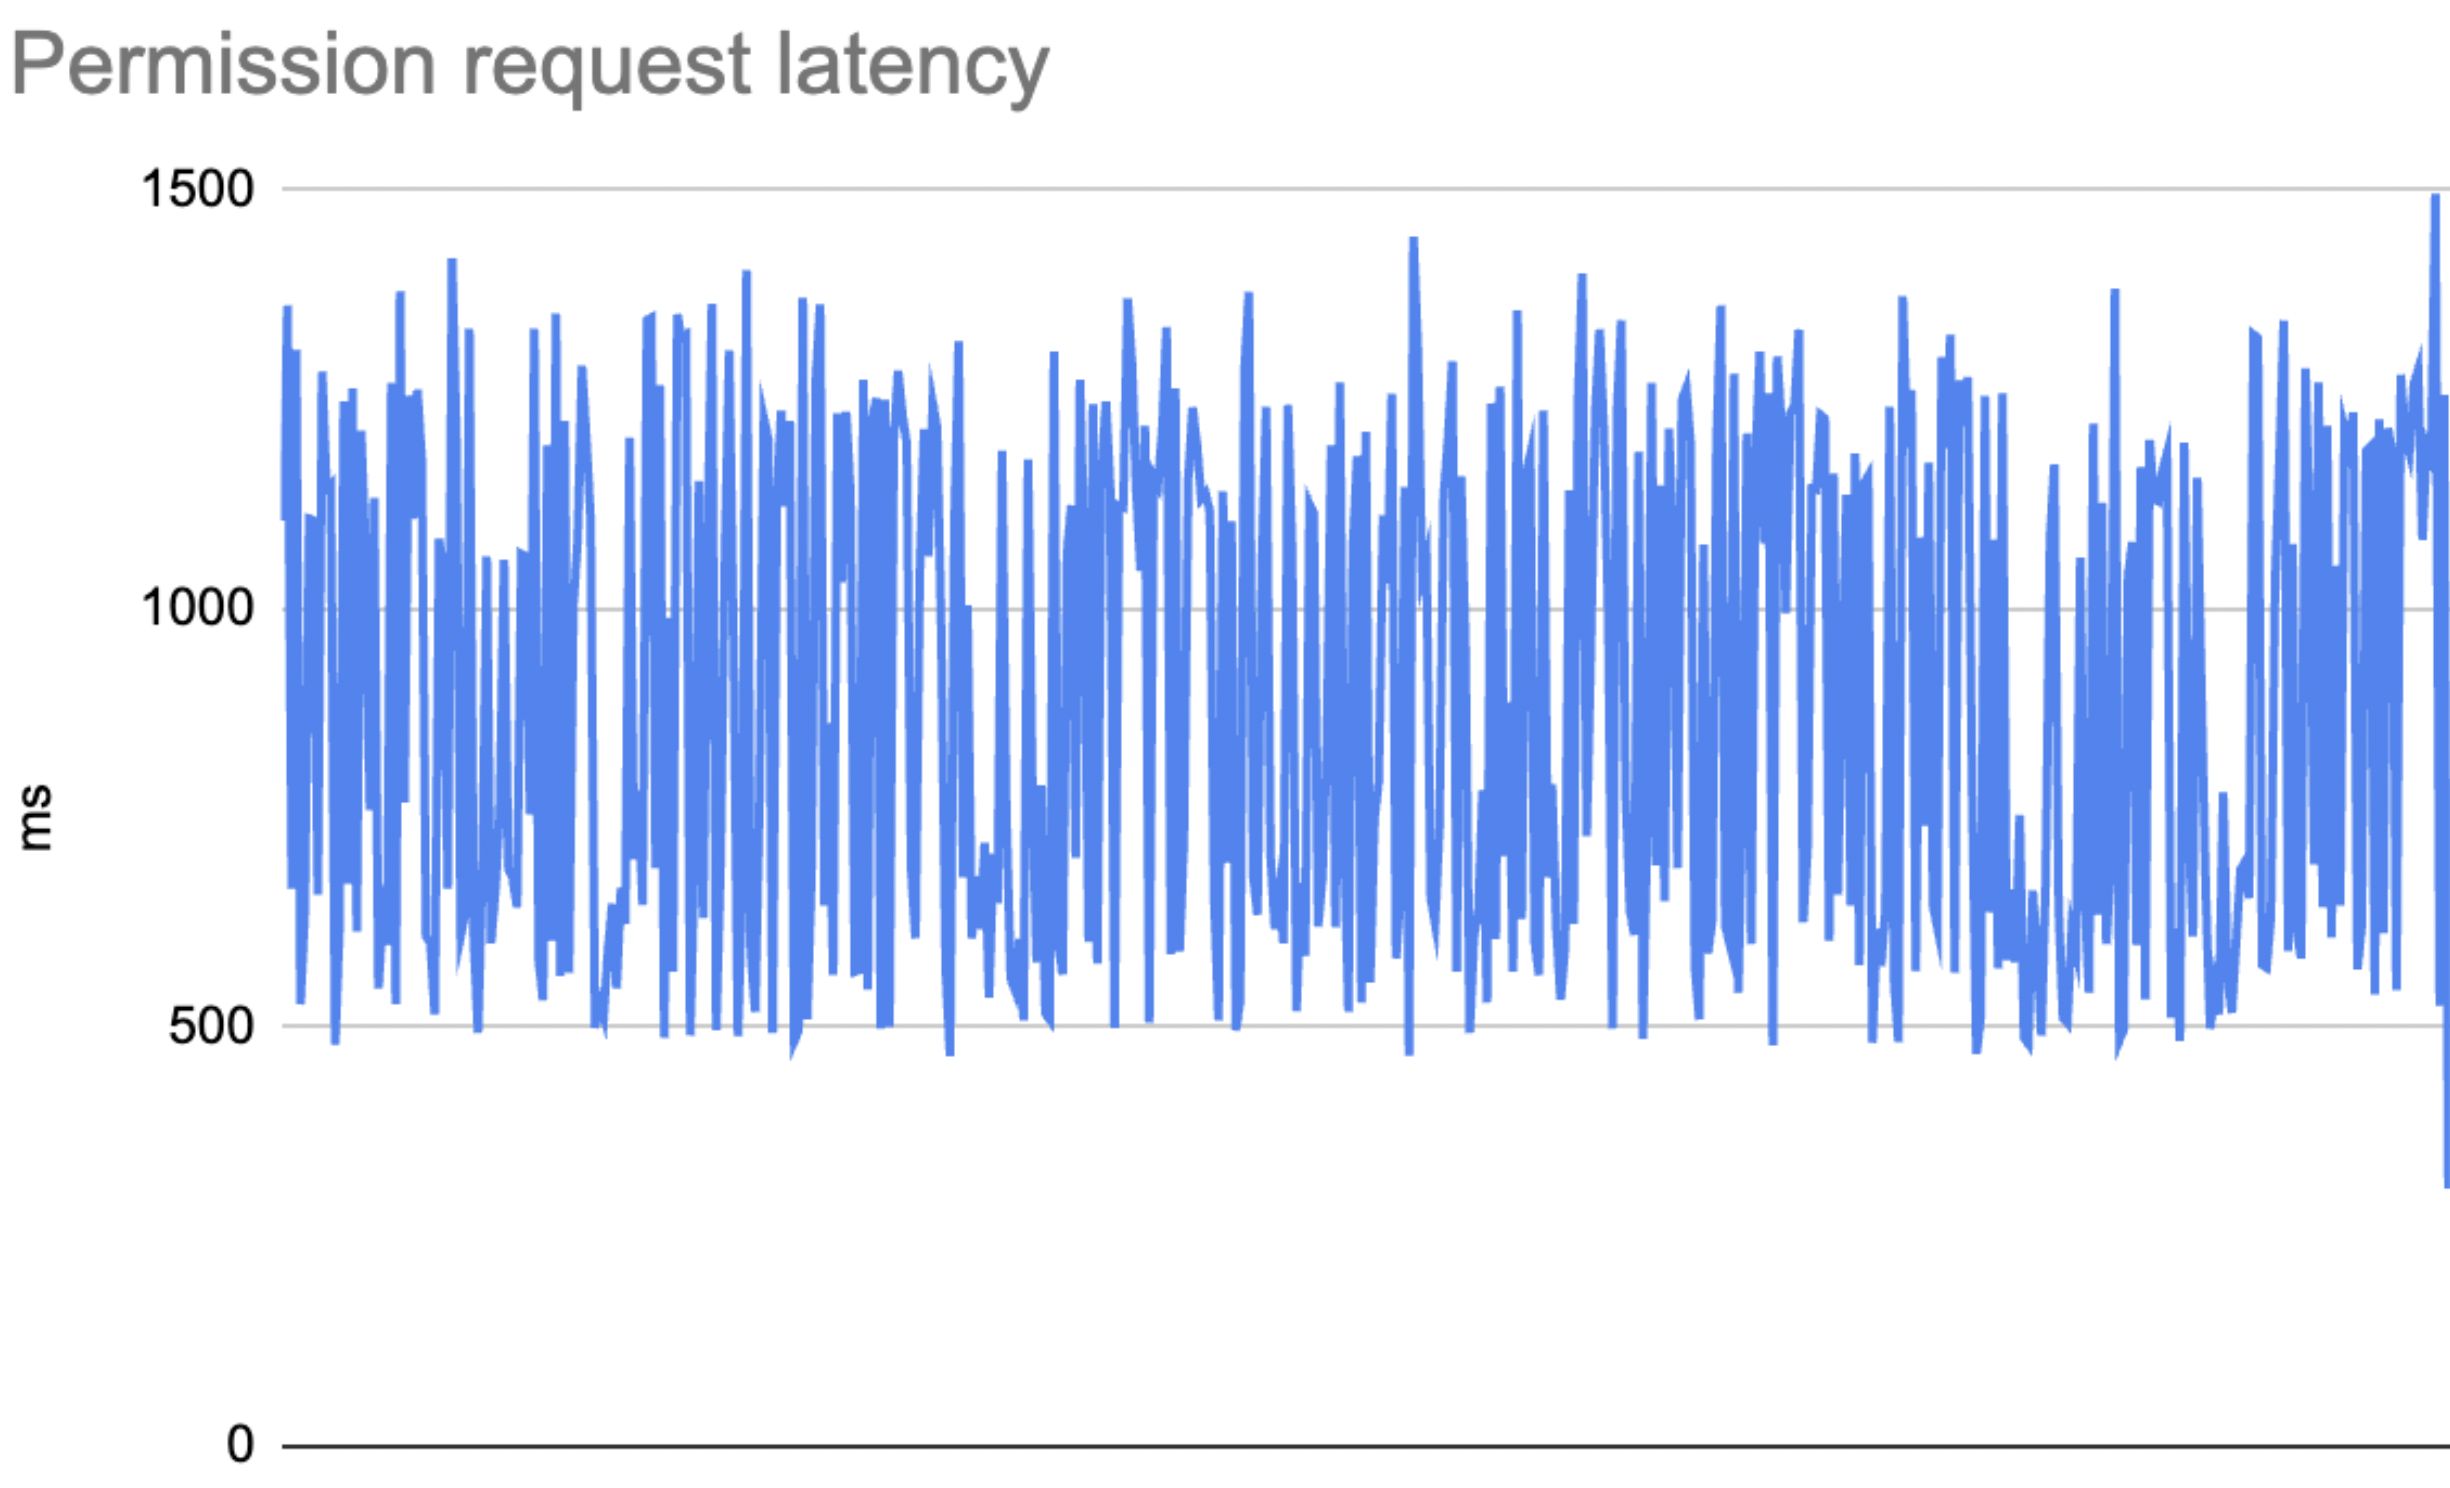
\includegraphics[width=\textwidth]{figsrc/result-p1.png}
    \caption{Latency of requesting permission over 500 times\label{fig:result-p1}}
\end{figure}

% build
\subsection{Phase 2: Build connection}
In build connection phase, we will measure the time from start sending MQTT recording command until recording server repsonds that it completes connection to streaming server as shown in Fig.~\ref{fig:result-p2-1}. Because recording command and reponse are both sent by MQTT, we use a local device to measure the time elapsed as shown in Fig.~\ref{fig:result-p2-2}. We will subtract the beginning time from the ending time to obtain latency. we repeat the experiment 200 times and each test has 1 minute interval. As shown in Fig.~\ref{fig:result-p2-3}, We see that average time elasped is 6408ms anf STD is 202. 

\begin{figure}[H]
    \centering
    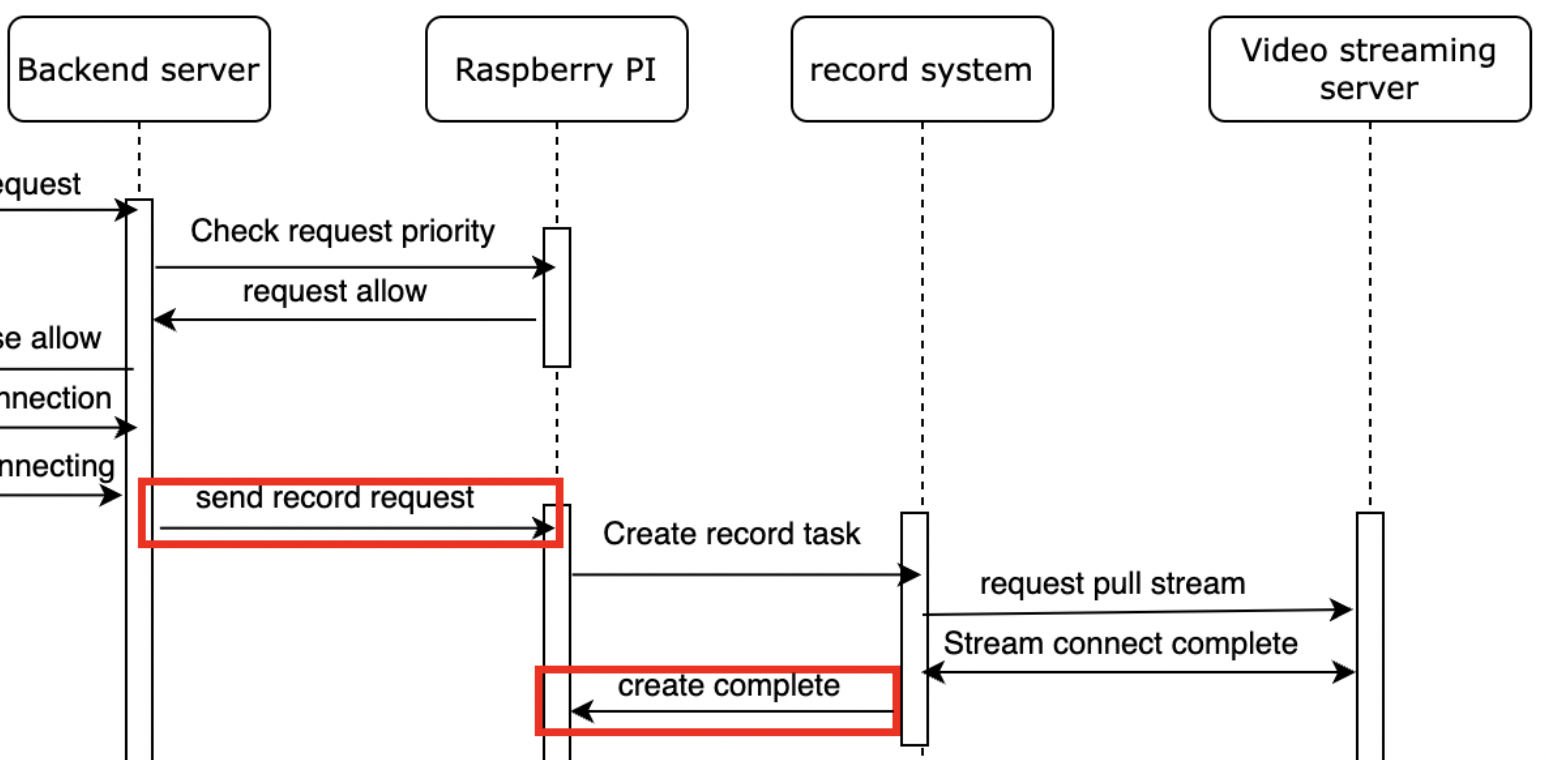
\includegraphics[width=\textwidth]{figsrc/result-p2-1.png}
    \caption{Starting point and ending point of phase 2 latency\label{fig:result-p2-1}}
\end{figure}

\begin{figure}[H]
    \centering
    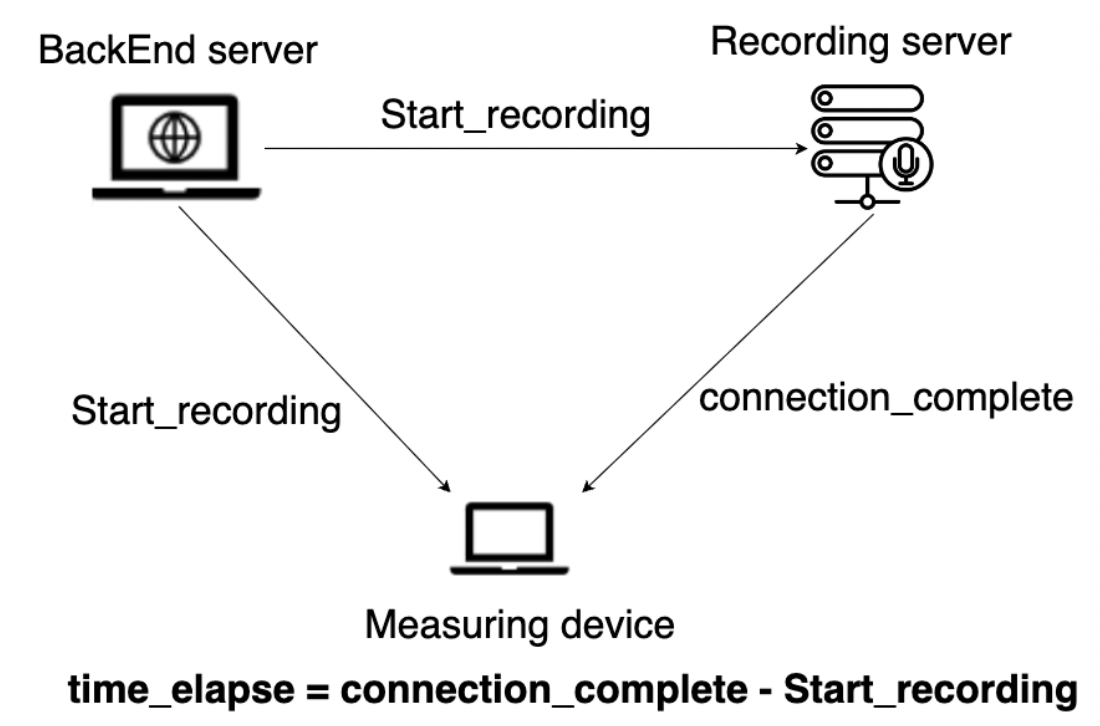
\includegraphics[width=\textwidth]{figsrc/result-p2-2.png}
    \caption{Get the MQTT message from 2 server then measure the time elapsed\label{fig:result-p2-2}}
\end{figure}

% result-p2-3
\begin{figure}[H]
    \centering
    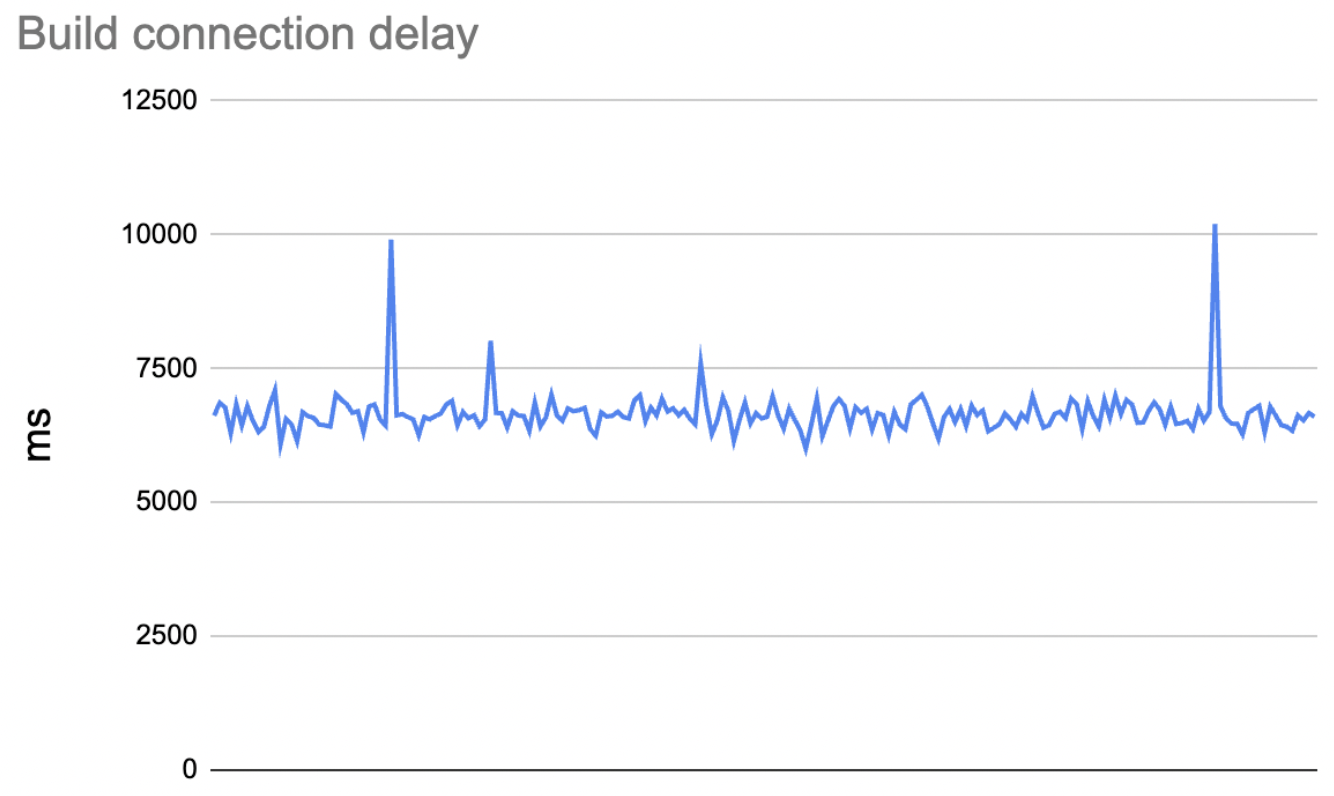
\includegraphics[width=\textwidth]{figsrc/result-p2-3.png}
    \caption{Latency of building connection\label{fig:result-p2-3}}
\end{figure}

% recording
\subsection{Phase 3: Recording}
We will ignore the recording phase since the latency is determined by how long the recording process takes.

% uplaod
\subsection{Phase 4: Uploading}
In uploading phase, we measure the latency by the network bandwith since our recording server is deployed in AWS EC2. The time elasped of uploading phase is detemined by the recording duration, or size of video file. Thus, we will determine our time elapsed by measuring how many MB can be sent per second(i.e how fast is the network bandwidth of AWS EC2). The video SPEC has resolution of 1920x1080, 15 FPS and video duration of 300s. The video file size is about 495MB. We repeat the experiment for 50 times. As shown in Fig.~\ref{fig:result-p4-1}, the average upload time is 7583ms. In other words, the bandwidth of AWS EC2 is 73.637MB per second or we can say that it takes average 25.277ms to upload every 1 second of video.

\begin{figure}[H]
    \centering
    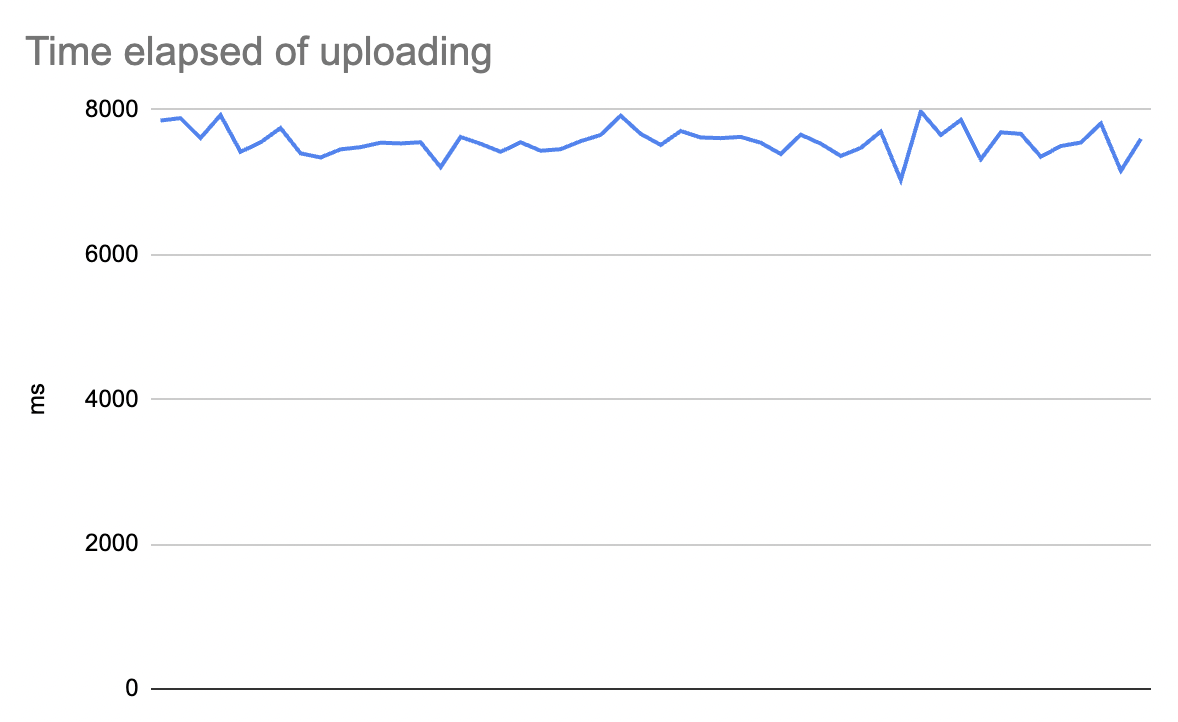
\includegraphics[width=\textwidth]{figsrc/result-p4-1.png}
    \caption{Latency of uploading\label{fig:result-p4-1}}
\end{figure}

\subsection{Observation}
Phase 1 has average delay of 902.856ms and Phase 2 has average delay of 6408ms. Phase 4 has average network bandwidth of 73.637MB/s. We can see that the bottleneck of the whole recording process is caused by building connection if the video file is small. But if the duration of video file exceeds 283s then upload time will be the bottleneck. As for user perspective, we expect that users concern more about the delay caused by Phase 1 + 2. So it may be better to improve the delay in Phase 1 + 2. Becuse it is usual that we care more about how long we have to wait to start the recording task.

\section{Scalability analysis}
We have shown the detail performance of single recording task. But what if there are multiple record tasks executing at the same time. Here we will show another bottleneck of the whole system. Recording process in recording server is the most resource-consuming task in the system. So we will test the performance of it by running different amount of tasks at the same time in recording server. As mentioned in Chapter 3, Our Recording server runs in AWS EC2. Operating System of EC2 VM is Ubuntu22.04. CPU is single Intel(R) Xeon(R) CPU E5-2676 v3 @ 2.40GH. RAM has size of 1 GB. As shown in Fig.~\ref{fig:result-scalability}, X-axis represents how many tasks are running at the same time. Y-axis represents the percentage of each components, such as Average CPU usage, Average RAM usage and Maximum CPU usage. Each number of task runs 5 times then calculate its average. We find that current server is only capable of running less than 5 task at the same time, if we don't want CPU usage exceed 70\% to make sure the stability of server. Although we have characteristic of automation and cloud-based in this system, scalability is what we need to improve in the future work.

\begin{figure}[H]
    \centering
    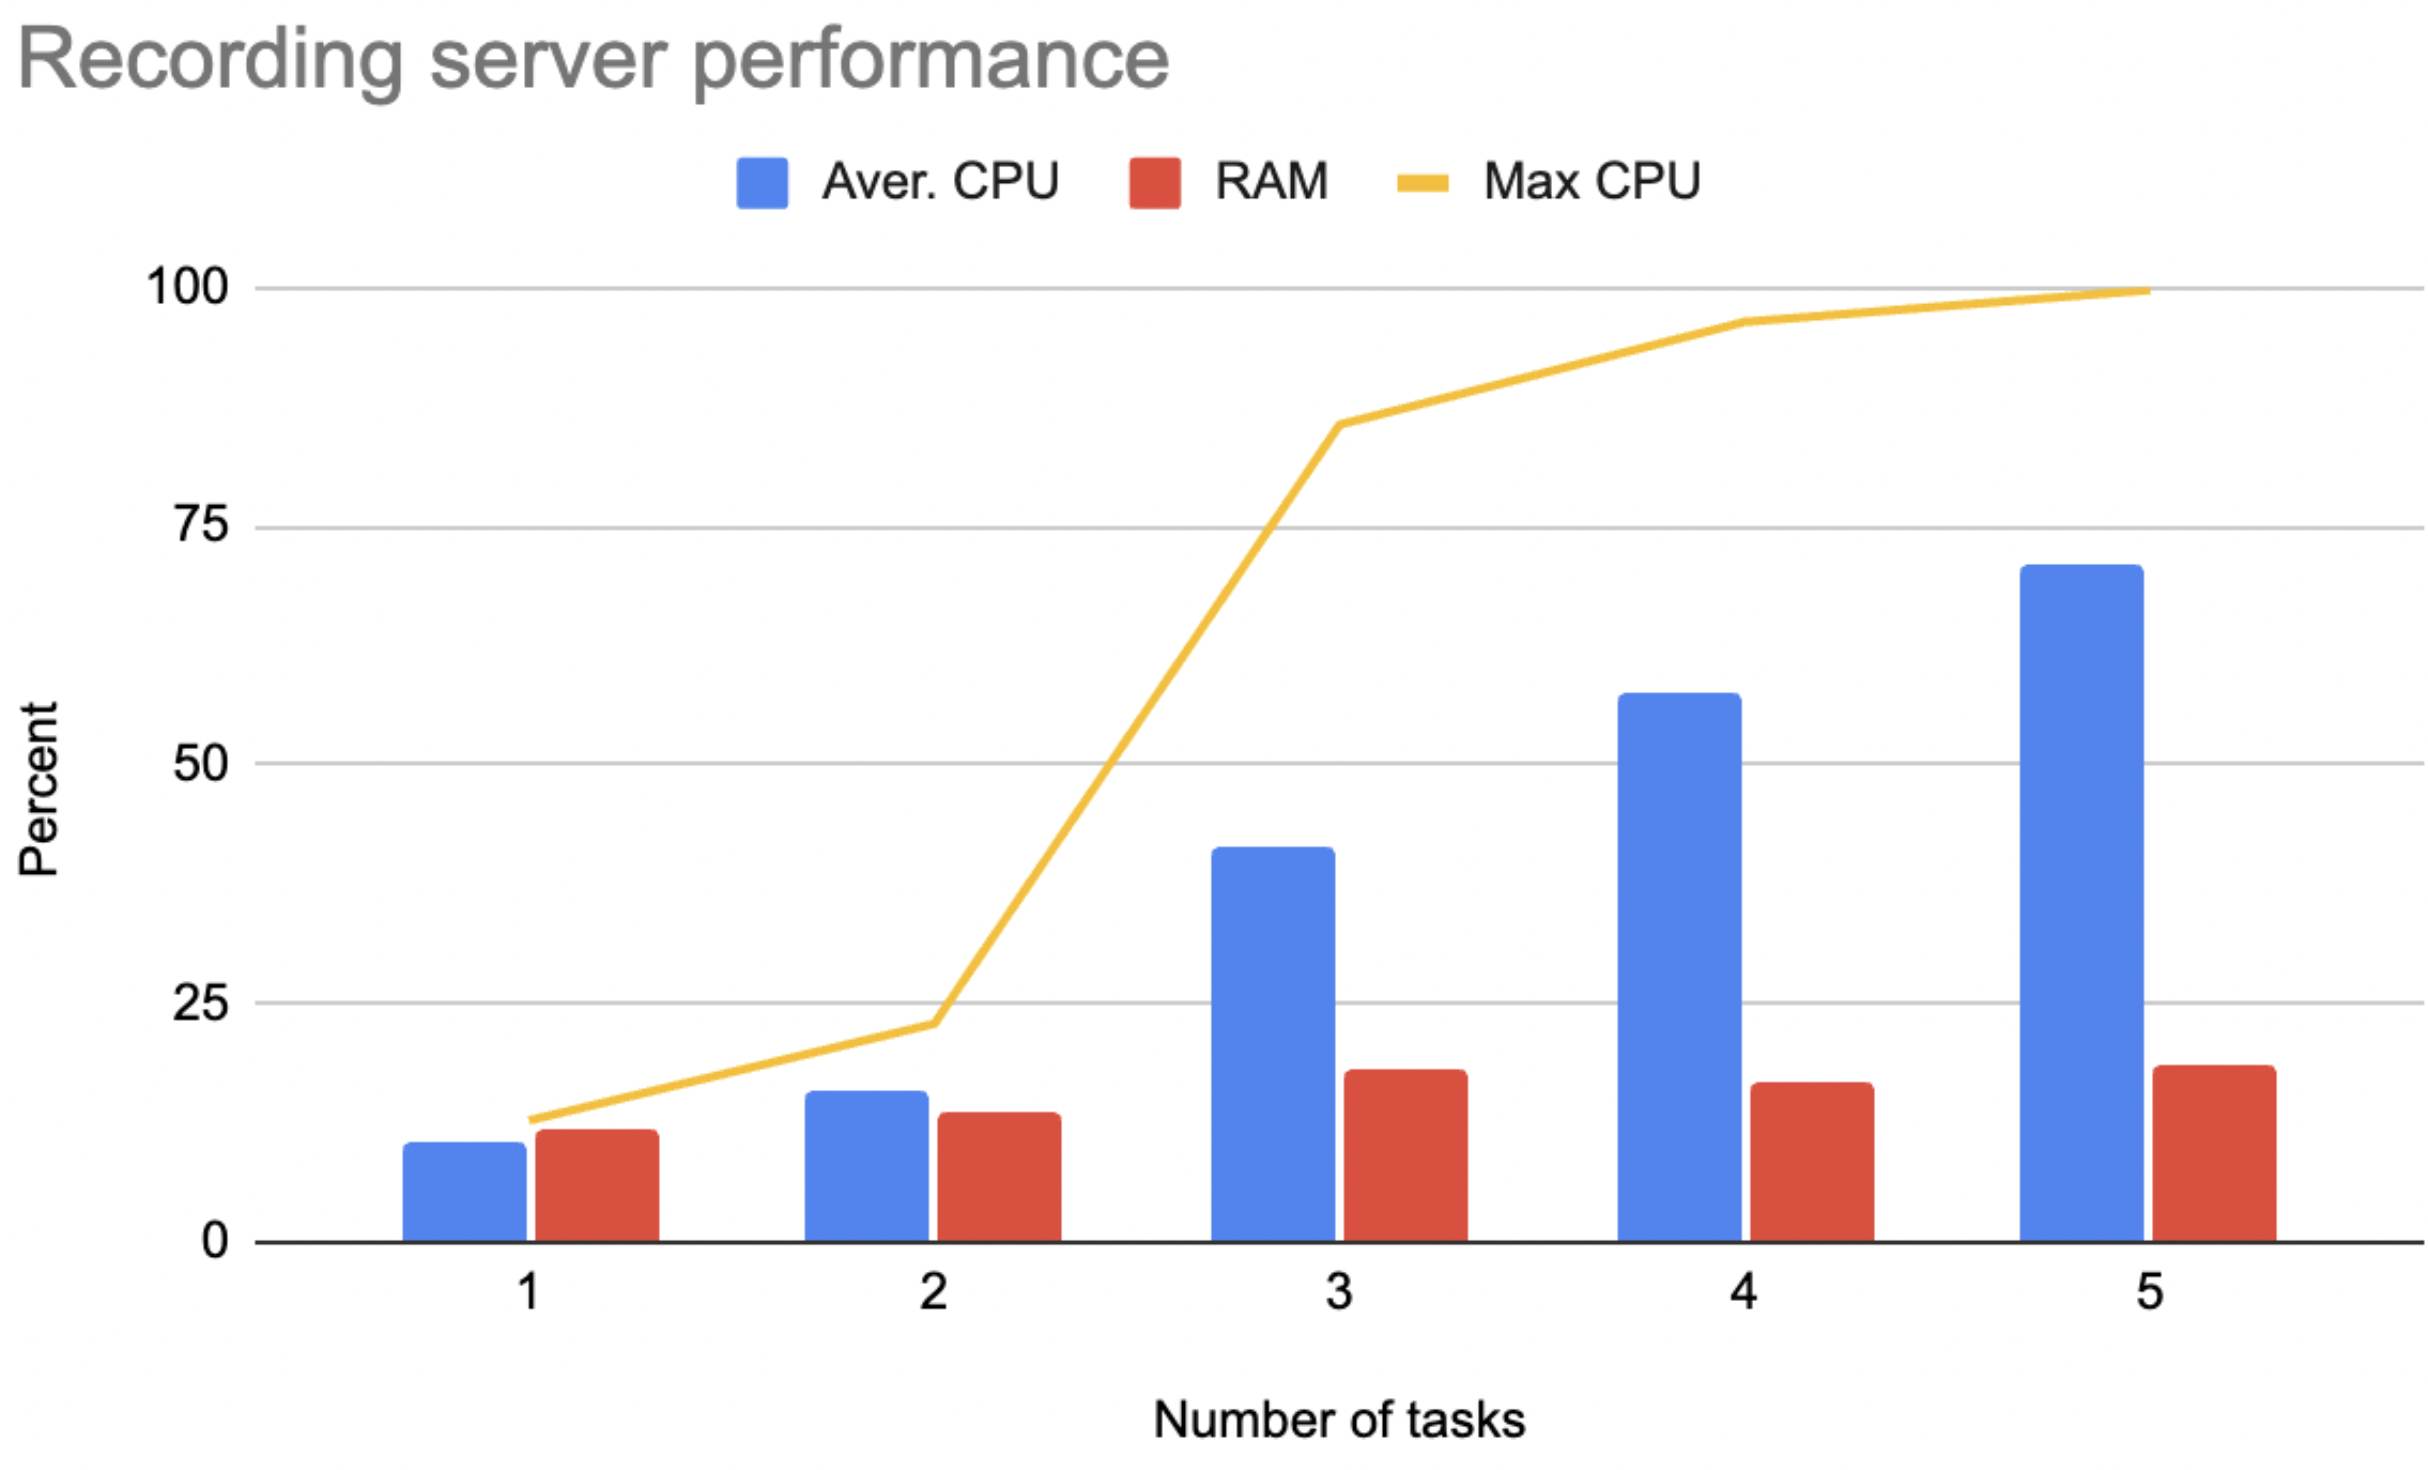
\includegraphics[width=\textwidth]{figsrc/result-scalability.png}
    \caption{Performance of multiple recording task\label{fig:result-scalability}}
\end{figure}

We also show the performace of phase 2 when they run different number of tasks at the same time in Fig.~\ref{fig:result-scale-2}. It shows that number of tasks running at the same time has little effect on phase 2. 

\begin{figure}[H]
    \centering
    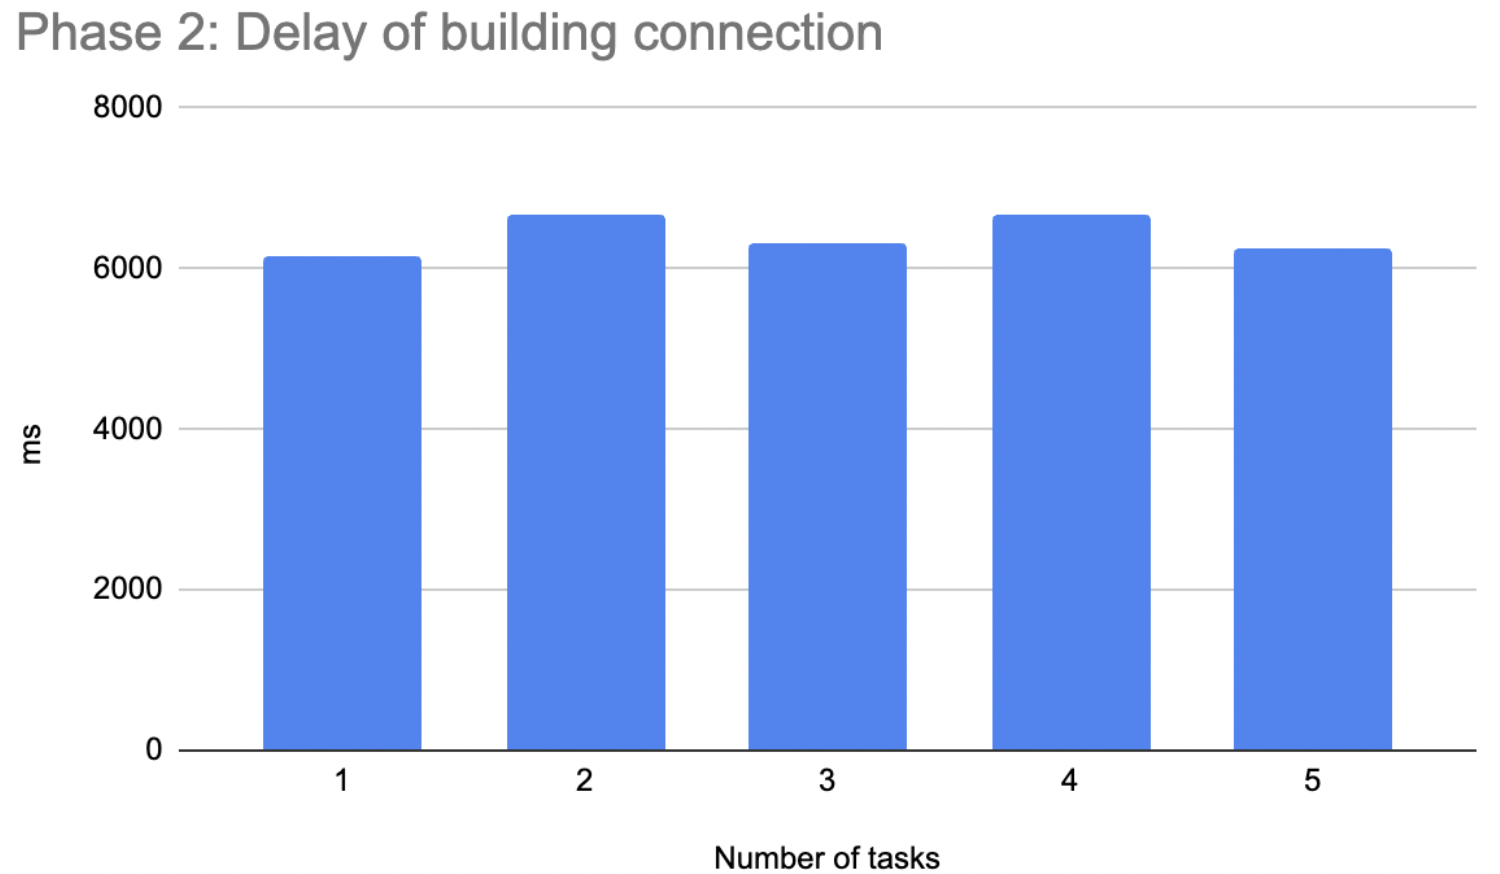
\includegraphics[width=\textwidth]{figsrc/result-scale-2.png}
    \caption{\label{fig:result-scale-2}}
\end{figure}

% 總結比較
% 可擴充性問題
